\section{System Model}
\label{system_model}

The vehicle--RSU--UAV--cloud network couples task service with communication,
motion, and energy availability. We specify these components separately so
that their interaction within a time slot is explicit.
Fig.~\ref{fig:network_slot} introduces the topology and execution order;
Fig.~\ref{fig:service_graph} follows a task through its service stages.
The models below define mobility, arrivals, offloading, radio service,
computation, queues, flight, and battery replenishment.
Section~\ref{problem_formulation} uses these definitions to state the
long-term control problem.

\subsection{Network Architecture and Time-Slot Model}
\label{subsec:network_model}
We consider a bounded rectangular service region
$\mathcal A\subset\mathbb R^2$. The node sets are
$\mathcal V=\{1,\ldots,V\}$ for vehicles,
$\mathcal R=\{1,\ldots,R\}$ for fixed RSUs, and
$\mathcal U=\{1,\ldots,U\}$ for rotary-wing UAV edge servers;
$c$ denotes a remote cloud. Vehicle and RSU positions are
$\boldsymbol p_v(t)=[x_v(t),y_v(t),0]^{\mathsf T}$ and
$\boldsymbol p_r=[x_r,y_r,0]^{\mathsf T}$, while UAV position and
velocity are $\boldsymbol p_k(t)\in\mathbb R^3$ and
$\boldsymbol u_k(t)\in\mathbb R^3$.

Time is slotted, $t\in\{0,1,\ldots\}$, with duration $\Delta>0$.
The state observed at the start of slot $t$ contains queues, eligible
task records, node positions, UAV velocities, physical battery charge,
virtual energy deficits, and current channel summaries. The slot order is:
\begin{enumerate}
\item observe start-of-slot state and generate control proposals;
\item repair proposals and execute radio, CPU, and flight service using
only work eligible at the start of the slot;
\item commit completed stage transfers at the boundary;
\item add external tasks and realized harvested energy; and
\item record completions, deadline crossings, cost, and the transition.
\end{enumerate}
Consequently, a transfer completed in slot $t$ can receive downstream
service no earlier than slot $t+1$.

\begin{figure*}[!t]
\centering
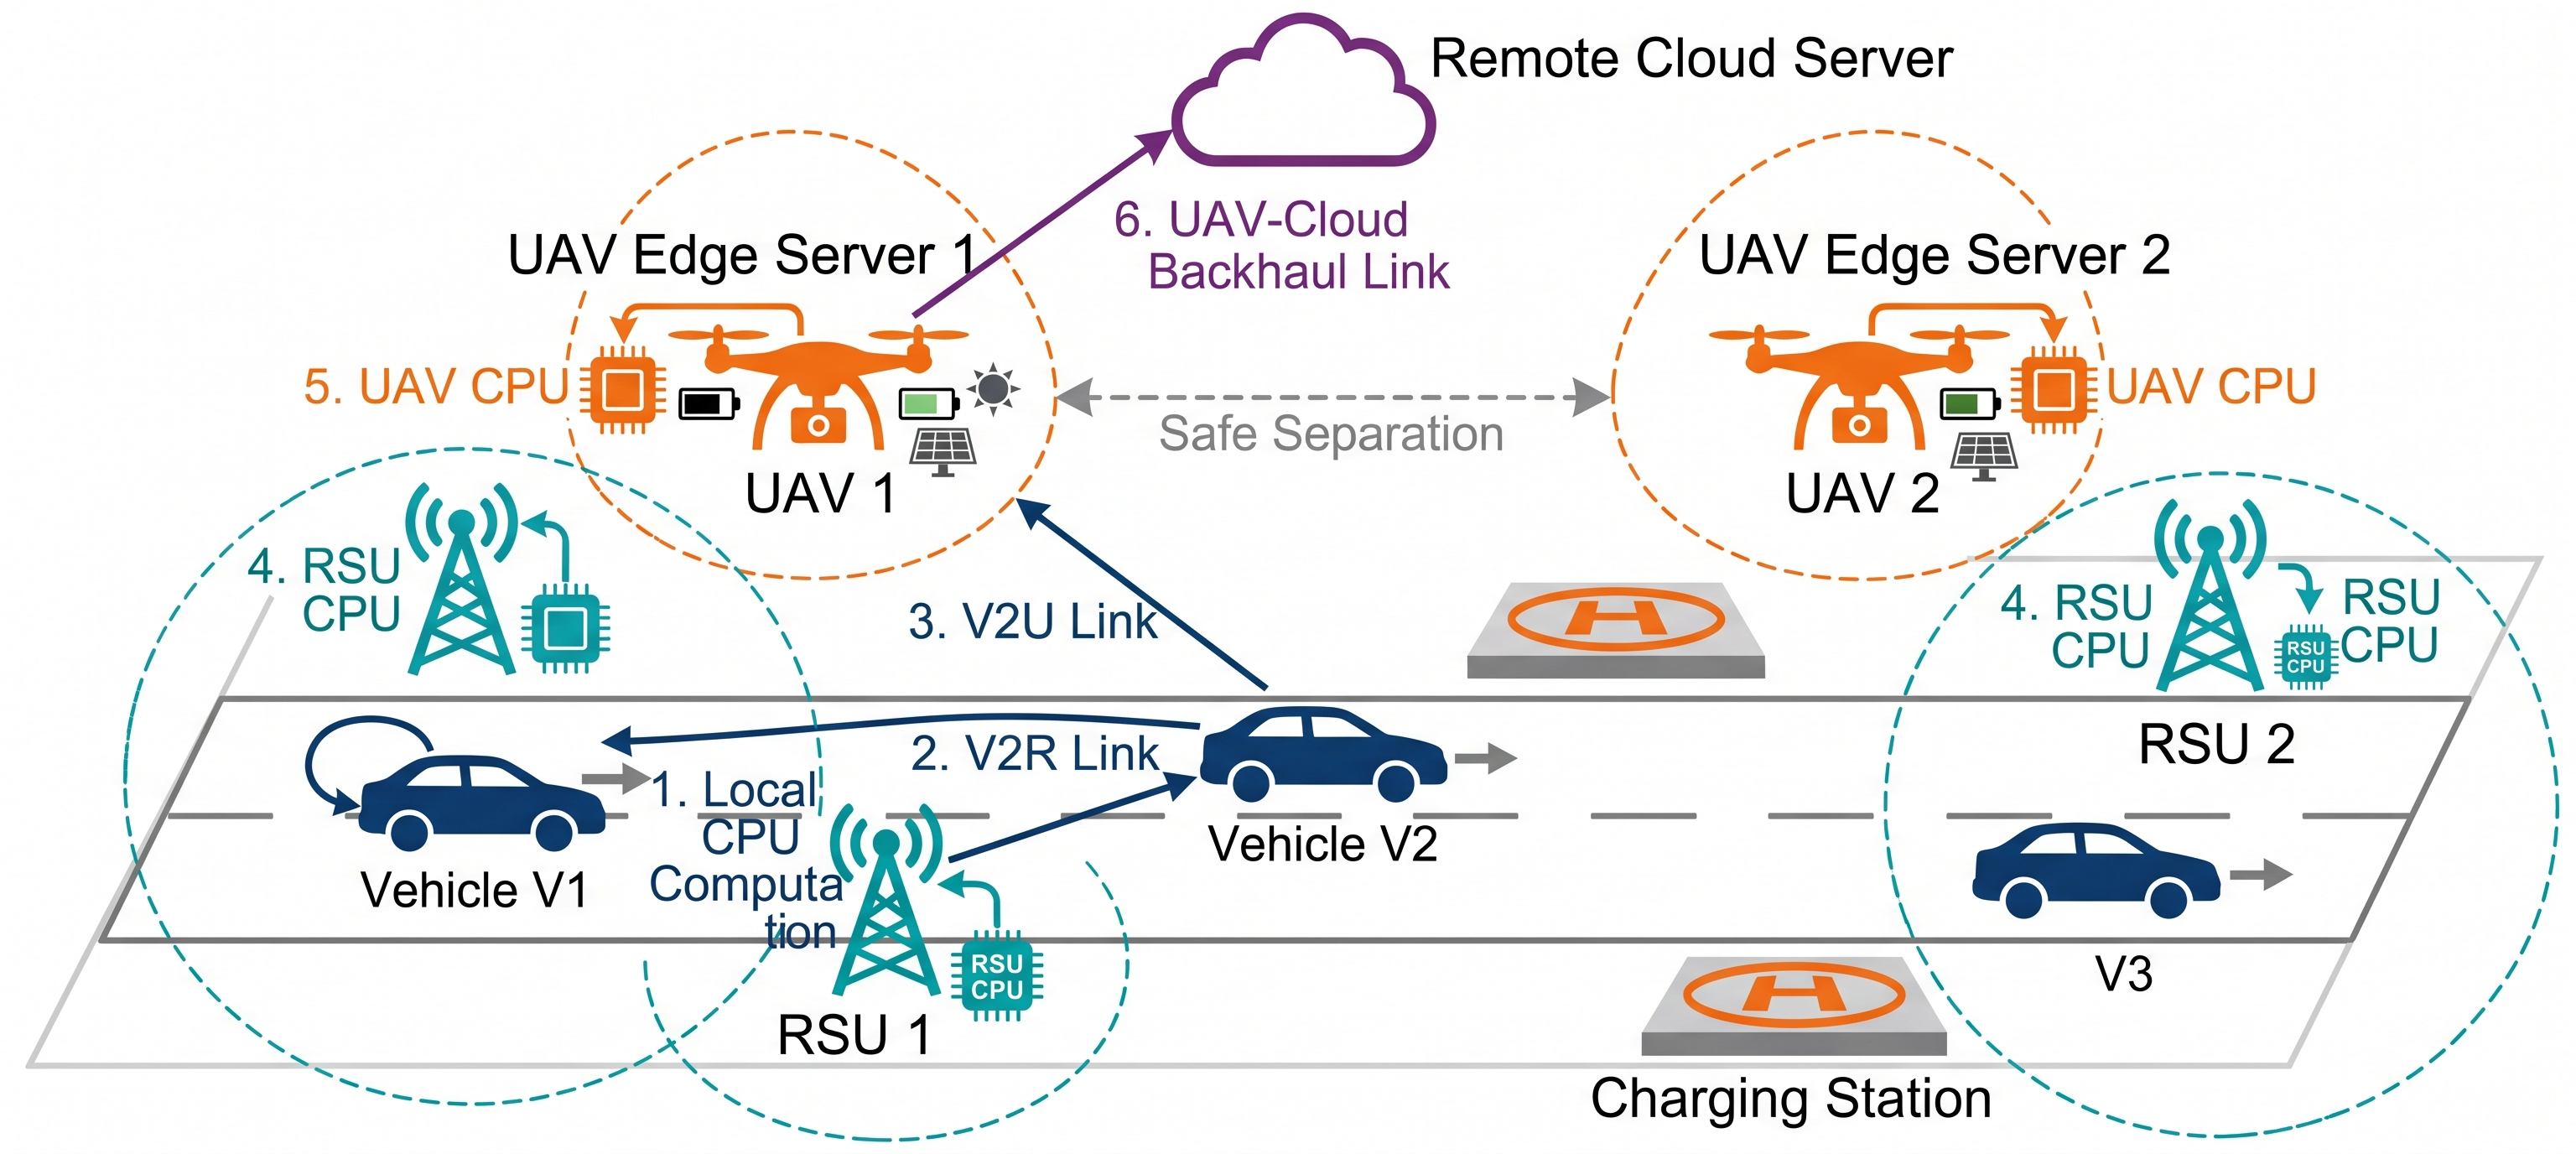
\includegraphics[width=0.94\textwidth]{Network architecture diagram.png}
\par\vspace{2pt}
{\footnotesize (a) Vehicle--RSU--UAV--cloud architecture.\par}
\vspace{5pt}
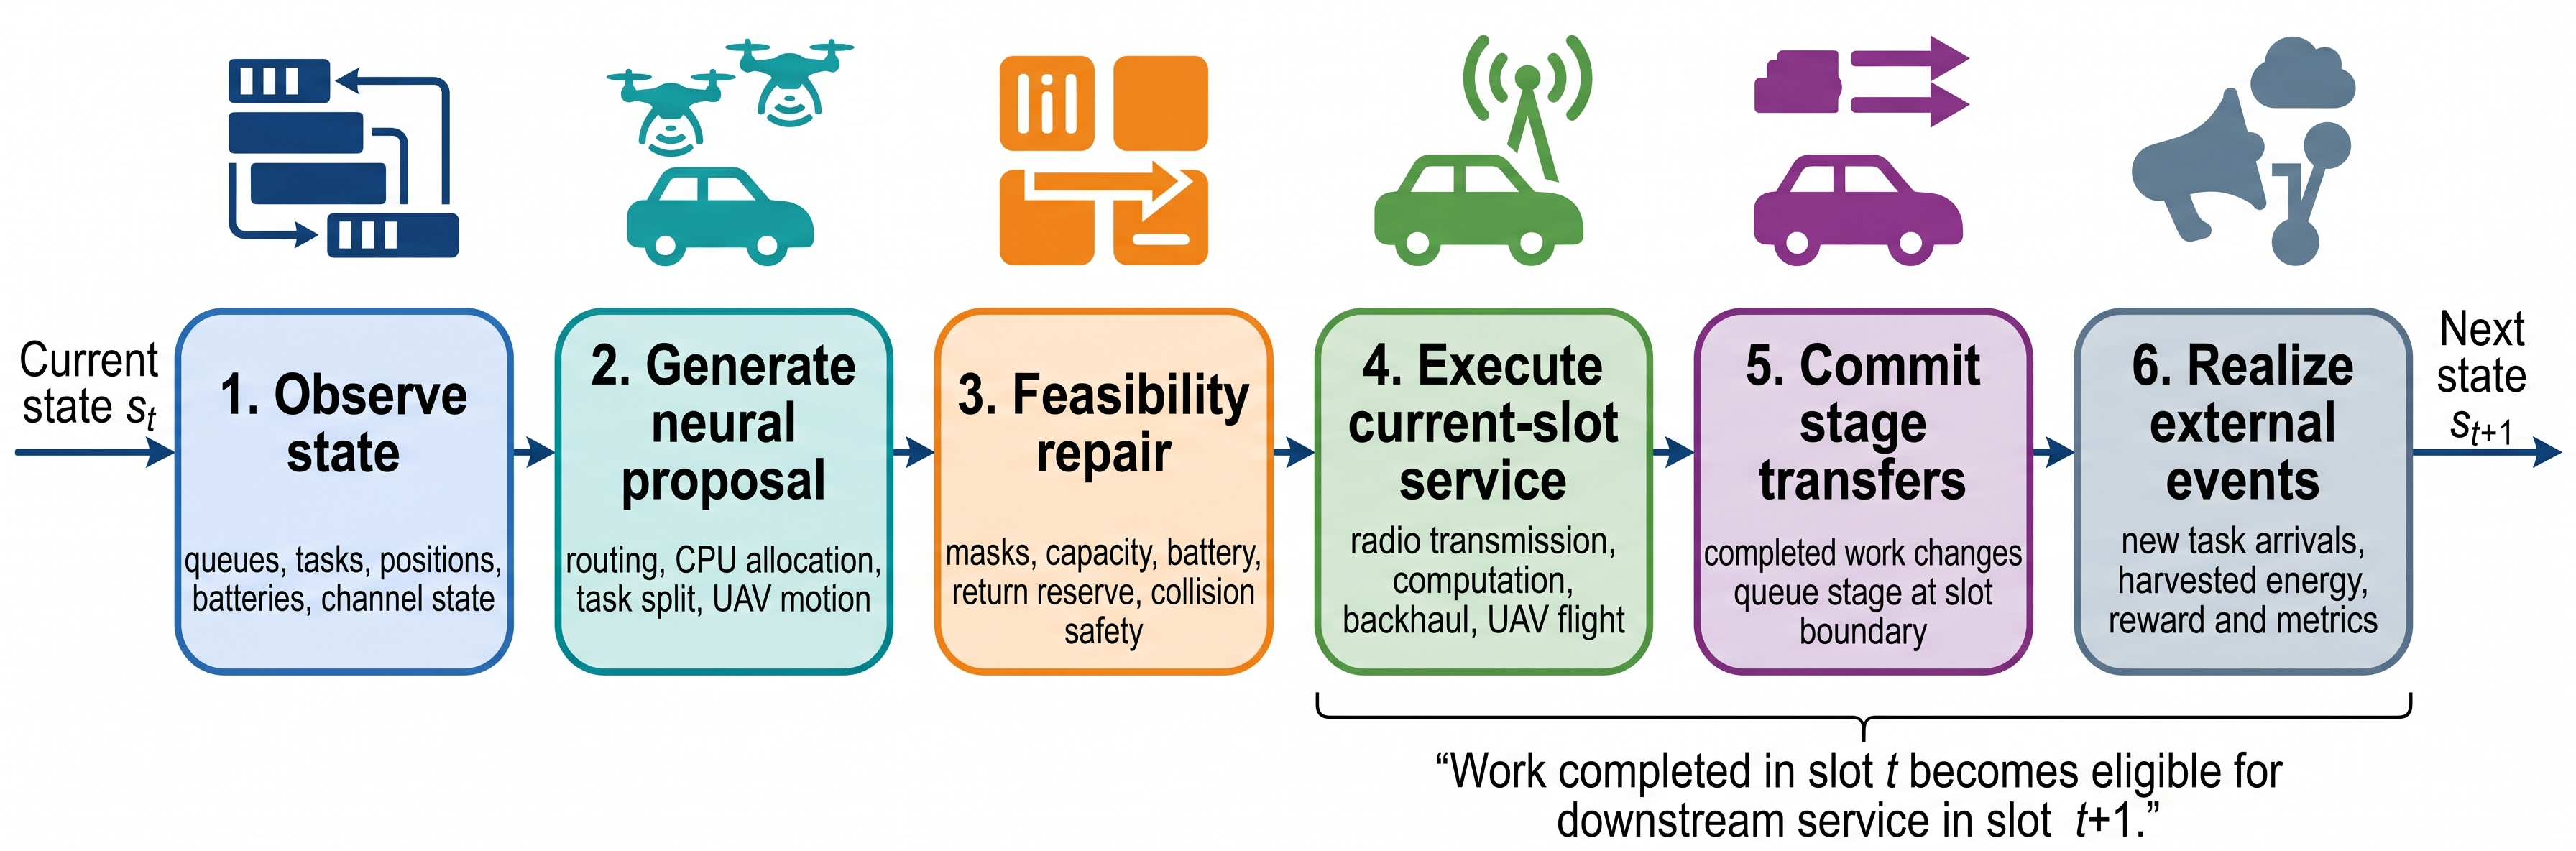
\includegraphics[width=0.96\textwidth]{Causal time-slot execution workflow.png}
\par\vspace{2pt}
{\footnotesize (b) Causal execution order within slot $t$.\par}
\caption{System architecture and causal slot execution. UAVs provide mobile
edge service, RSUs provide fixed edge capacity, and UAV-bound work may retain
a finite cloud branch. Harvest and external arrivals are committed only after
current-slot service and expenditure.}
\label{fig:network_slot}
\end{figure*}

\begin{figure*}[t]
\centering
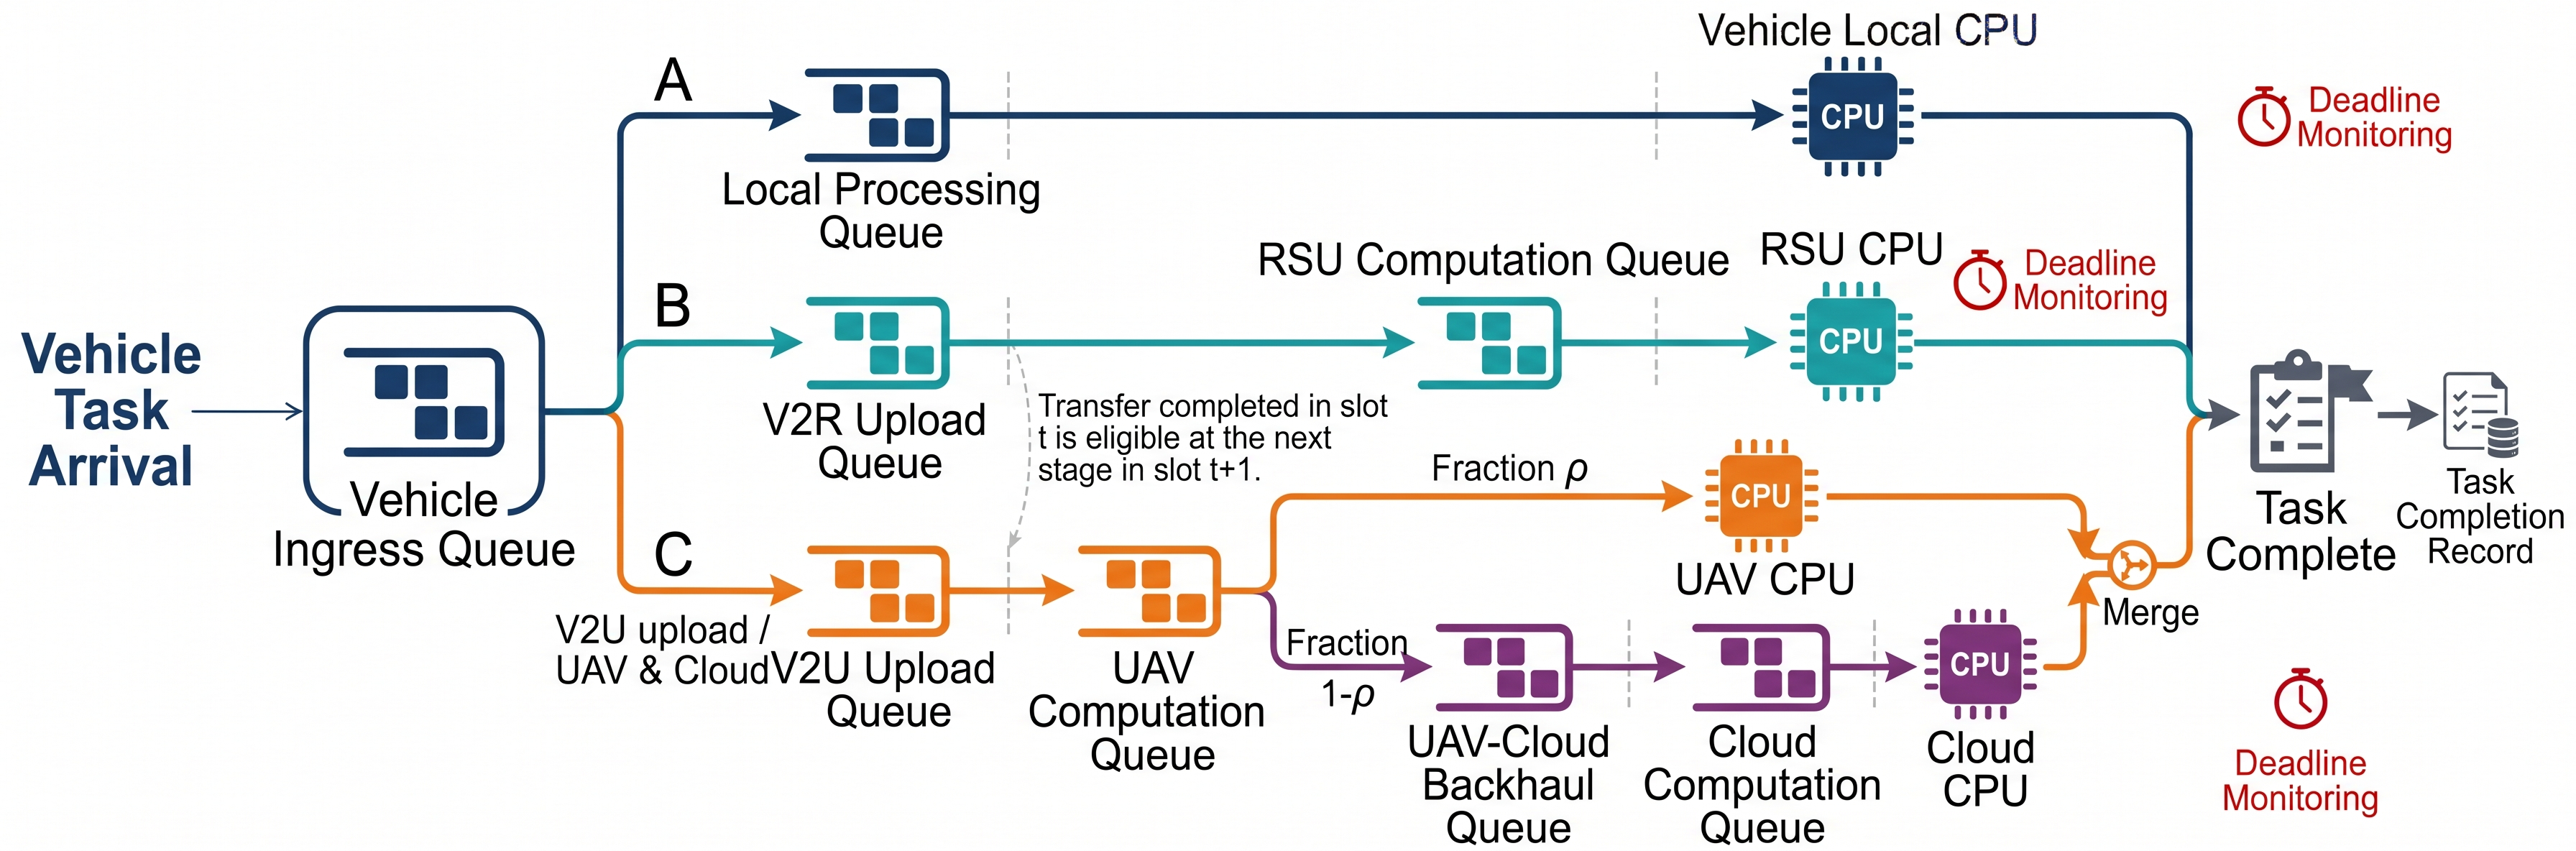
\includegraphics[width=0.96\textwidth]{End-to-end task lifecycle and queue mode.png}
\caption{End-to-end task service graph. Every box is represented by a
persistent task or queue stage. Transfers committed at one boundary
become eligible at the following boundary.}
\label{fig:service_graph}
\end{figure*}

The core architecture has no direct vehicle-to-cloud or RSU-to-cloud
route, no inter-UAV task migration, and no reassignment after
dispatch. Radio transmit powers are fixed and uplinks use orthogonal
bandwidth. These choices isolate the routing, CPU, split, and
trajectory decisions studied here.

\begin{table*}[t]
\centering
\caption{Principal system notation.}
\label{tab:notation}
\renewcommand{\arraystretch}{1.12}
\begin{tabular}{p{0.13\textwidth}p{0.31\textwidth}p{0.13\textwidth}p{0.30\textwidth}}
\hline
\textbf{Symbol} & \textbf{Meaning} & \textbf{Symbol} & \textbf{Meaning}\\
\hline
$\Delta$ & Slot duration &
$\ell_i$ & Immutable task specification\\
$b_i,c_i,\chi_i$ & Input bits, CPU cycles, cycles per bit &
$a_i,d_i$ & Arrival time and deadline allowance\\
$Q_j(t)$ & Equivalent-cycle backlog of stage queue $j$ &
$A_j(t),S_j(t)$ & Realized queue arrival and service\\
$W_{ih}(t),R_{ih}(t)$ & Link bandwidth and transmission rate &
$f_n(t),w_{in}(t)$ & CPU frequency and task share\\
$B_k(t),H_k(t)$ & Physical UAV charge and harvested energy &
$Z_k(t)$ & Virtual net-energy deficit\\
$\boldsymbol p_v,\boldsymbol p_r,\boldsymbol p_k$ &
Vehicle, RSU, and UAV positions &
$\rho_i$ & UAV-local workload fraction\\
\hline
\end{tabular}
\end{table*}

\subsection{Vehicle Mobility and Coverage Model}
Synthetic vehicles follow declared road polylines. Let
$\boldsymbol r_v(s)$ map route distance $s\in[0,L_v]$ to a 3-D road
coordinate, and let $\nu_v(t)\ge0$ be vehicle speed. Route progress obeys
\begin{equation}
\begin{aligned}
s_v(t+1)&=\mathscr R_v\!\left(
s_v(t)+\sigma_v(t)\nu_v(t)\Delta\right),\\
\boldsymbol p_v(t)&=\boldsymbol r_v(s_v(t)),
\end{aligned}
\label{eq:vehicle_motion}
\end{equation}
where $\sigma_v(t)\in\{-1,1\}$ is direction and
$\mathscr R_v$ either wraps a loop or reflects progress at a route
endpoint. For recorded SUMO experiments, Eq.~\eqref{eq:vehicle_motion}
is replaced by the complete sampled trace
$\boldsymbol p_v(t)=\boldsymbol p_v^{\mathrm{trace}}(t)$; missing
vehicle frames are rejected rather than interpolated.

The three-dimensional distance from vehicle $v$ to edge node
$n\in\mathcal R\cup\mathcal U$ and its horizontal component are
\begin{equation}
d_{vn}(t)=\|\boldsymbol p_v(t)-\boldsymbol p_n(t)\|,\qquad
d_{vn}^{\mathrm H}(t)=
\|[\boldsymbol p_v(t)-\boldsymbol p_n(t)]_{1:2}\|.
\label{eq:distances}
\end{equation}
Coverage indicators are
$\mathbf 1\{d_{vr}^{\mathrm H}\le D_R\}$ for RSUs and
$\mathbf 1\{d_{vk}^{\mathrm H}\le D_U\}$ for UAVs. A destination is
masked whenever it is outside coverage, inactive, returning, or lacks
an admissible energy contingency.

\subsection{Task Generation, Lifecycle, and Offloading Model}
\label{subsec:task_model}
\subsubsection{Task Arrival and Persistent Record Model}
At slot $t$, vehicle $v$ generates $A_v^{\mathrm{task}}(t)$ jobs. The
controlled synthetic benchmark uses
\begin{equation}
\begin{aligned}
A_v^{\mathrm{task}}(t)&\sim
\operatorname{Poisson}(\lambda_v(t)),\\
b_i&\in[b_{\min},b_{\max}],\quad
c_i\in[c_{\min},c_{\max}],\\
d_i&\in[d_{\min},d_{\max}],
\end{aligned}
\label{eq:task_arrival}
\end{equation}
with bounded independent draws recorded once in a scenario trace.
Low-load, near-capacity, overload, and surge cases differ through
$\lambda_v(t)$. Each task has immutable record
\begin{equation}
\ell_i=(i,v(i),b_i,c_i,a_i,d_i,\zeta_i),\qquad
\chi_i=\frac{c_i}{b_i},
\label{eq:task_record}
\end{equation}
where $\zeta_i\in\{0,1\}$ identifies whether the job is partitionable.

\subsubsection{Destination Selection and Partitioning Model}
Let $h_i(t)$ denote holding in ingress and let $x_i^L(t)$,
$x_{ir}^R(t)$, and $x_{ik}^U(t)$ be local, RSU, and UAV dispatch
indicators. Before dispatch,
\begin{equation}
h_i(t)+x_i^L(t)+\sum_{r\in\mathcal R}x_{ir}^R(t)
 +\sum_{k\in\mathcal U}x_{ik}^U(t)=1,
\quad x,h\in\{0,1\}.
\label{eq:destination}
\end{equation}
If $h_i=1$, the task remains in ingress. Once a non-hold choice is
made, its destination and dispatch time are fixed.

For a UAV destination, the complete input is first uploaded to the
chosen UAV. The UAV executes fraction $\rho_i$ and forwards the
remainder to the cloud:
\begin{equation}
c_i^U=\rho_i c_i,\qquad
c_i^c=(1-\rho_i)c_i,\qquad
b_i^{\mathrm{bh}}=(1-\rho_i)b_i.
\label{eq:split}
\end{equation}
For indivisible work, $\rho_i=1$. For partitionable work,
$0\le\rho_i\le1$ is fixed at dispatch. Completion requires every
nonempty branch followed by merge delay $\tau_i^{\mathrm{merge}}$.

\subsubsection{End-to-End Completion and Delay Model}
With actual completion time $f_i^{\mathrm{done}}$, response time and
deadline success are
\begin{equation}
T_i=f_i^{\mathrm{done}}-a_i,\qquad
\delta_i=\mathbf 1\{T_i\le d_i\}.
\label{eq:actual_latency}
\end{equation}
The simulator records a miss when a task first crosses its deadline and
continues to track its remaining work. If the trace ends before completion,
the task is reported as censored; no completion latency is imputed.

\subsection{Communication and OFDMA Service Model}
\subsubsection{Vehicle-to-RSU Terrestrial Channel Model}
For a vehicle--RSU link, the deterministic large-scale gain is
\begin{equation}
g_{vr}^{R}(t)=g_0
\max\{d_{vr}(t),d_{\min}^{\mathrm{ch}}\}^{-\alpha_R},
\label{eq:rsu_gain}
\end{equation}
where $g_0$ is reference gain and $\alpha_R$ is the terrestrial
path-loss exponent.

\subsubsection{Vehicle-to-UAV Air-to-Ground Channel Model}
For a vehicle--UAV link, elevation angle and LoS probability are
\begin{equation}
\begin{aligned}
\vartheta_{vk}(t)&=
\frac{180}{\pi}\tan^{-1}\!\left(
\frac{|z_k(t)-z_v(t)|}
{\max\{d_{vk}^{\mathrm H}(t),d_{\min}^{\mathrm{ch}}\}}\right),\\
p_{vk}^{\mathrm{LoS}}(t)&=
\left[1+a_{\mathrm L}
\exp\{-b_{\mathrm L}[\vartheta_{vk}(t)-a_{\mathrm L}]\}\right]^{-1}.
\end{aligned}
\label{eq:los}
\end{equation}
The mean aerial gain is
\begin{equation}
\begin{aligned}
g_{vk}^{U}(t)={}&g_0
\max\{d_{vk}(t),d_{\min}^{\mathrm{ch}}\}^{-\alpha_U}\\
&\times\left[p_{vk}^{\mathrm{LoS}}\eta_{\mathrm L}
+(1-p_{vk}^{\mathrm{LoS}})\eta_{\mathrm N}\right],
\end{aligned}
\label{eq:uav_gain}
\end{equation}
where $\eta_{\mathrm L}=10^{-L_{\mathrm L}/10}$ and
$\eta_{\mathrm N}=10^{-L_{\mathrm N}/10}$ represent additional LoS
and NLoS losses.

\subsubsection{OFDMA Rate and Transmission-Service Model}
For link $h$ with assigned bandwidth $W_{ih}(t)$, fixed vehicle power
$P_v^{\mathrm{tx}}$, and gain $g_{ih}(t)$, the rate is
\begin{equation}
R_{ih}(t)=W_{ih}(t)\log_2\!\left(
1+\frac{P_v^{\mathrm{tx}}g_{ih}(t)}
{N_0W_{ih}(t)+I_{ih}(t)}\right).
\label{eq:rate}
\end{equation}
Orthogonal operation gives $I_{ih}=0$ and
$\sum_iW_{ih}\le W_h^{\max}$.

The shared deterministic scheduler assigns priority
\begin{equation}
\begin{aligned}
\pi_{ih}(t)&=q_{ih}^{\mathrm{eq}}(t)
\left[1+\min\left\{\frac{\operatorname{age}_i(t)}{d_i},
\kappa_{\mathrm{age}}\right\}\right],\\
W_{ih}(t)&=W_h^{\max}
\frac{\pi_{ih}(t)}{\sum_{\ell\in\mathcal E_h}\pi_{\ell h}(t)}.
\end{aligned}
\label{eq:ofdma}
\end{equation}
over eligible links $\mathcal E_h$, with task ID resolving exact ties.
Here $q_{ih}^{\mathrm{eq}}$ is the link backlog in equivalent cycles.
A transfer of $s_{ih}^{\mathrm{tr}}$ equivalent cycles must obey
\begin{equation}
\sum_i\frac{s_{ih}^{\mathrm{tr}}(t)}{\chi_i}
\le\Delta R_h(t).
\label{eq:radio_capacity}
\end{equation}
When coverage is lost, the link provides no service in that slot. Its
untransmitted bits remain in the original upload queue.

\subsection{Computation, Backhaul, and Queueing Model}
\subsubsection{Persistent Multi-Stage Queue Model}
The queue set $\mathcal J$ contains ingress, V2R/V2U upload,
receive/staging, local/RSU/UAV compute, UAV backhaul, cloud receive,
and cloud compute stages. Bit queues are converted only for drift
accounting: $b$ residual bits of task $i$ equal $\chi_i b$ cycles.

For each queue $j$, realized service $S_j(t)$ and arrivals $A_j(t)$ give
\begin{equation}
Q_j(t+1)=Q_j(t)-S_j(t)+A_j(t),\qquad
0\le S_j(t)\le Q_j(t).
\label{eq:queue}
\end{equation}
If $F_{ab}(t)$ moves equivalent work from stage $a$ to stage $b$,
then it appears as $-F_{ab}$ in the source increment and $+F_{ab}$ in
the destination increment. Thus
\begin{equation}
\sum_{j\in\mathcal J}Q_j(t+1)=
\sum_{j\in\mathcal J}Q_j(t)+A^{\mathrm{ext}}(t)-C^{\mathrm{final}}(t),
\label{eq:conservation}
\end{equation}
up to explicitly logged branch creation and merge bookkeeping.
Internal routing cannot destroy work; only final computation removes it.

\subsubsection{CPU Service and Processor-Sharing Model}
At compute node $n$, frequency $f_n$, task shares $w_{in}$, and ready
residual work $c_{in}^{\mathrm{elig}}$ satisfy
\begin{equation}
\begin{aligned}
0&\le f_n(t)\le f_n^{\max},\\
w_{in}(t)&\ge0,\qquad \sum_iw_{in}(t)\le1,\\
0\le s_{in}^{\mathrm{cpu}}(t)&\le
\min\{c_{in}^{\mathrm{elig}}(t),\Delta f_n(t)w_{in}(t)\}.
\end{aligned}
\label{eq:cpu_capacity}
\end{equation}
Unused capacity from a task that finishes early is redistributed among
remaining positive-share tasks. Local vehicle and cloud scheduling,
together with the RSU clock frequency, are fixed in the core experiments.
RSU task shares and both UAV frequency and task shares are controlled.

\subsubsection{UAV Backhaul and Cloud-Service Model}
The cloud branch of UAV task $i$ first traverses a finite backhaul:
\begin{equation}
\sum_{i\in\mathcal B_k(t)}
\frac{s_{ik}^{\mathrm{bh}}(t)}{\chi_i}
\le\Delta R_k^{\mathrm{bh}},
\qquad
\sum_i s_{ic}^{\mathrm{cpu}}(t)\le\Delta f_c.
\label{eq:cloud_capacity}
\end{equation}
Backhaul completion releases $(1-\rho_i)c_i$ cycles into cloud
computation at the next boundary. The task finishes only after the UAV
and cloud branches, if nonempty, have both completed.

\subsubsection{Queue-Stability Target}
The desired strong-stability condition is
\begin{equation}
\limsup_{T\to\infty}\frac1T\sum_{t=0}^{T-1}
\mathbb E[Q_j(t)]<\infty,\qquad j\in\mathcal J.
\label{eq:stability}
\end{equation}
This condition is meaningful only for stabilizable offered load.
Overload experiments intentionally report queue growth.

\subsection{UAV Movement and Collision-Avoidance Model}
Let horizontal speed be $v_k^{\mathrm H}$, azimuth $\theta_k$, and
vertical speed $v_k^z$. The velocity and position update are
\begin{equation}
\begin{aligned}
\boldsymbol u_k(t)&=
\begin{bmatrix}
v_k^{\mathrm H}\cos\theta_k&
v_k^{\mathrm H}\sin\theta_k&v_k^z
\end{bmatrix}^{\mathsf T},\\
\boldsymbol p_k(t+1)&=\boldsymbol p_k(t)+\Delta\boldsymbol u_k(t).
\end{aligned}
\label{eq:uav_motion}
\end{equation}
Admissible motion obeys speed, climb/descent, map, altitude, and
acceleration bounds:
\begin{equation}
\begin{aligned}
\|\boldsymbol u_k(t)\|&\le v_k^{\max},\\
-v_k^{\mathrm{down}}&\le v_k^z(t)\le v_k^{\mathrm{up}},\\
\|\boldsymbol u_k(t)-\boldsymbol u_k(t-1)\|&\le a_k^{\max}\Delta.
\end{aligned}
\label{eq:flight_bounds}
\end{equation}
Every pair of airborne UAVs must remain separated along the complete
linear slot trajectories:
\begin{equation}
\min_{\tau\in[0,\Delta]}
\|\boldsymbol p_k(t)+\tau\boldsymbol u_k(t)
-\boldsymbol p_l(t)-\tau\boldsymbol u_l(t)\|
\ge d_{\mathrm{safe}}.
\label{eq:collision}
\end{equation}
The controller also preserves sufficient stopping distance to map and
altitude boundaries. A verified return/landing plan is a sequence of
segments satisfying the same limits, terminating at a declared landing
site with near-zero velocity.

\subsection{UAV and Infrastructure Energy-Consumption Models}
Fig.~\ref{fig:energy_safety_overview} summarizes the UAV energy ledger,
replenishment paths, flight constraints, and the return-reserve rule. The
laser-transfer branch is optional and is not active in the reported
stochastic-harvesting benchmark.

\begin{figure*}[!t]
\centering
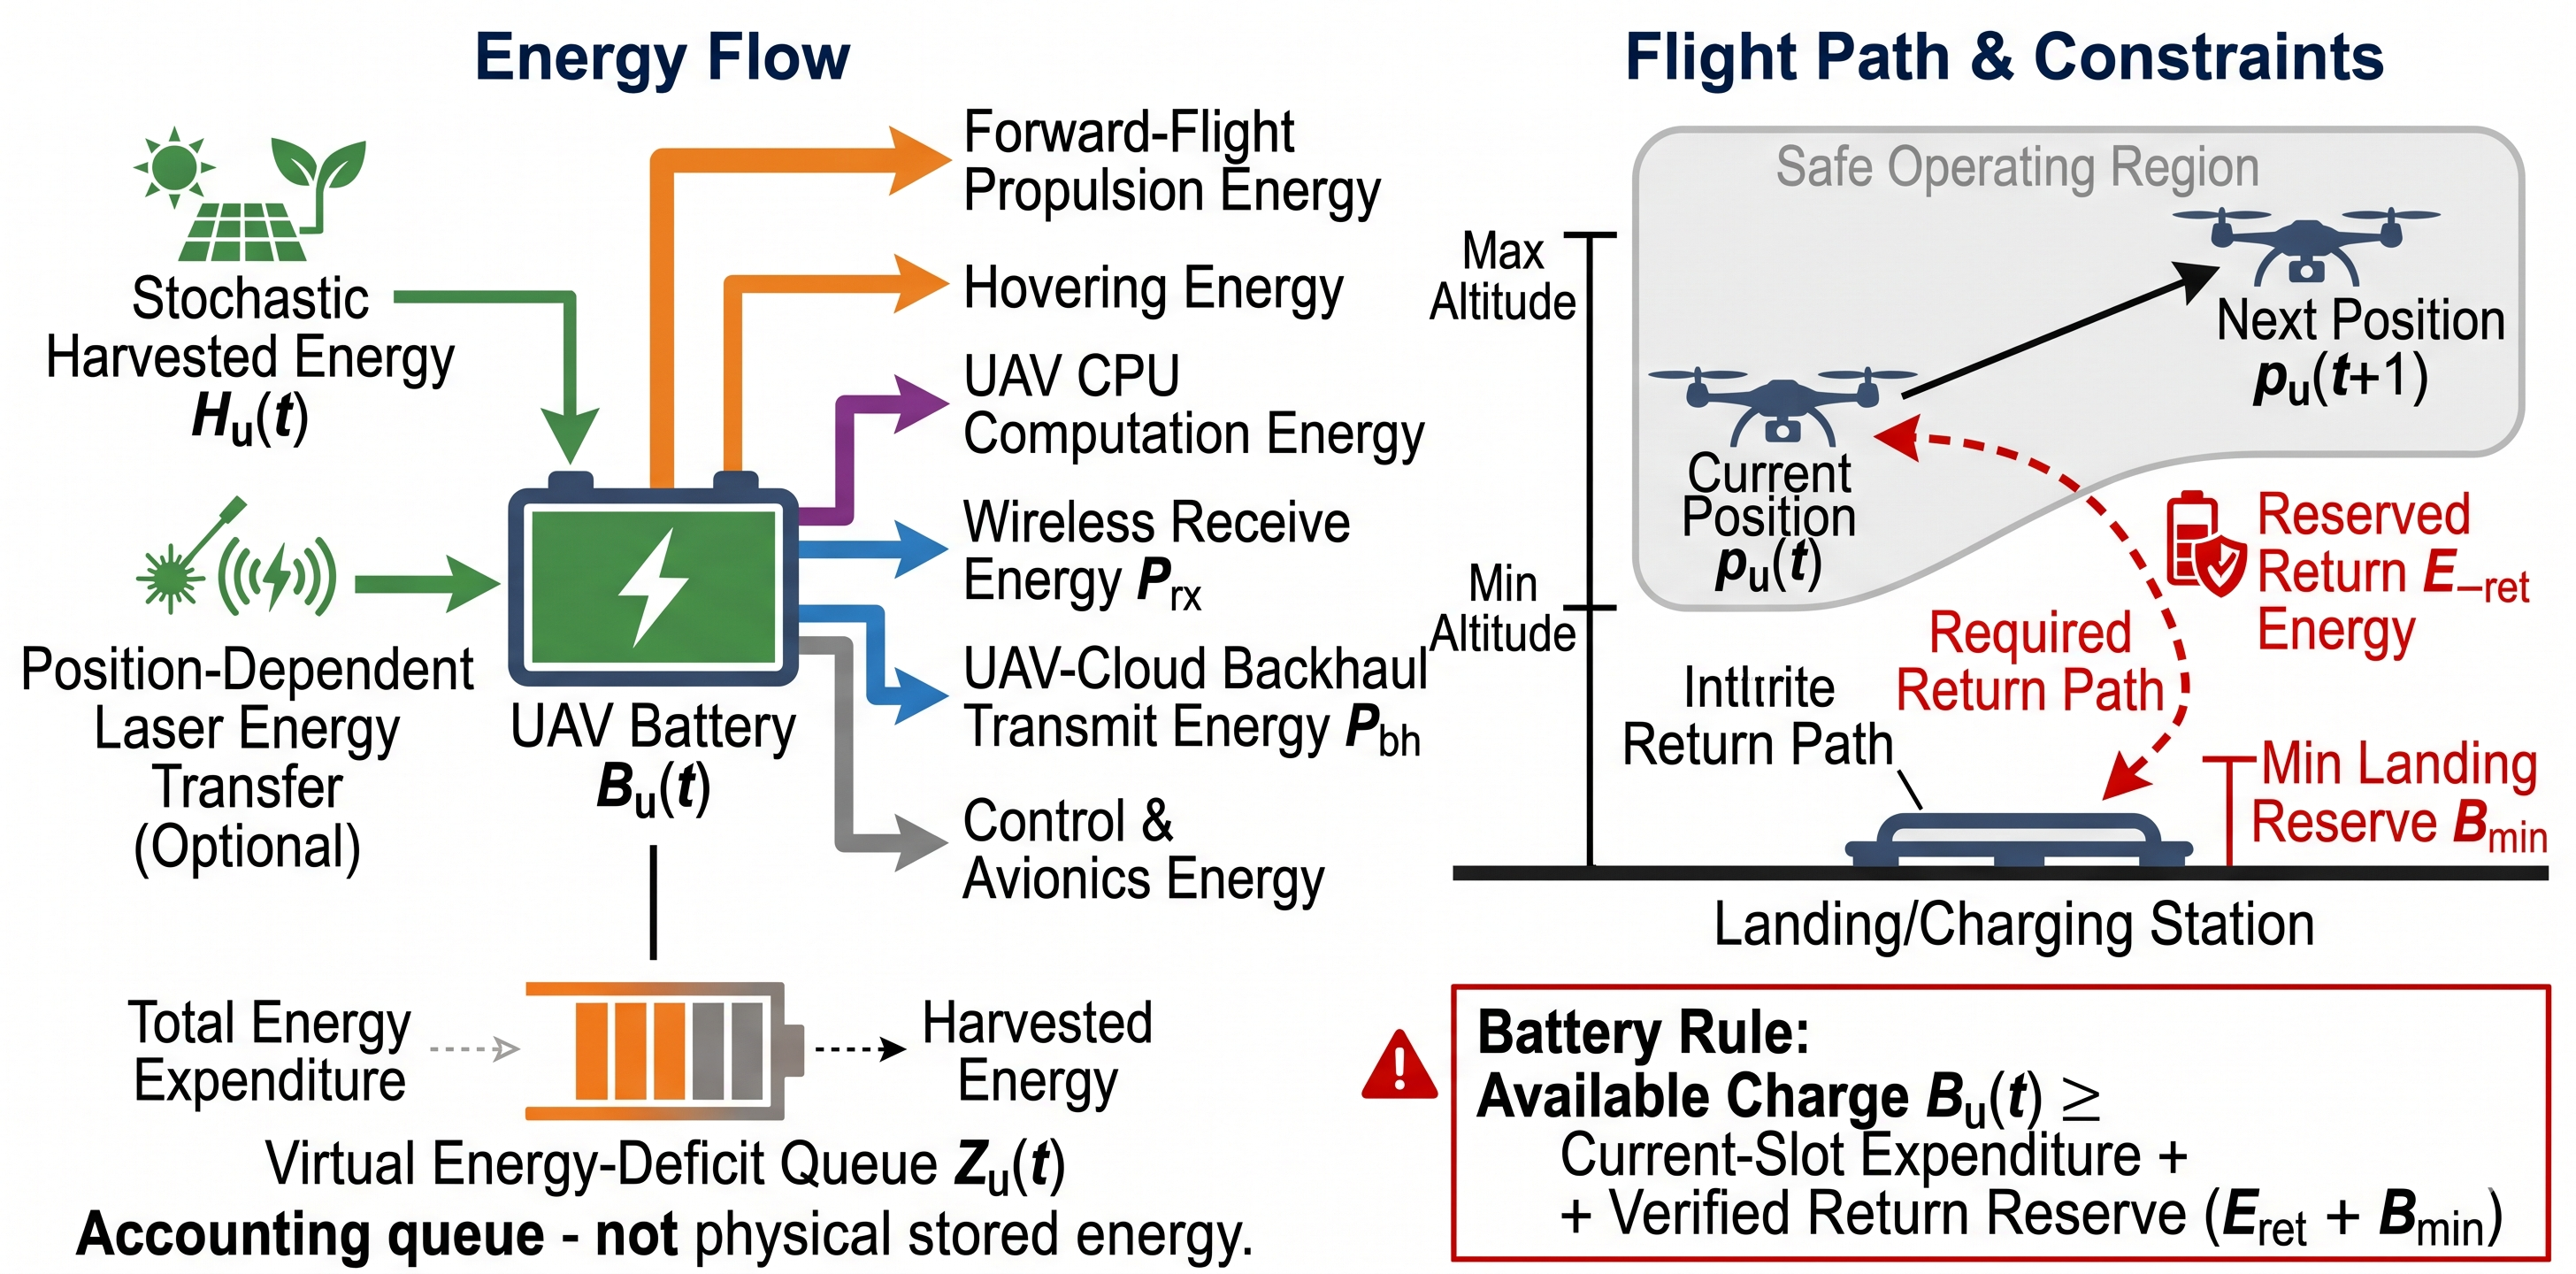
\includegraphics[width=0.94\textwidth]{UAV energy, harvesting, and return-reserve model.png}
\caption{UAV energy, harvesting, and return-reserve model. Physical battery
charge supplies propulsion, computation, communication, and control energy;
normal service is admitted only when current expenditure and a verified
return or landing reserve remain feasible. The virtual deficit is an
accounting queue rather than stored energy.}
\label{fig:energy_safety_overview}
\end{figure*}

\subsubsection{Rotary-Wing Flight and Hovering-Energy Model}
The propulsion ledger explicitly separates motion from hovering, following
the energy-accounting organization in~\cite{talukdar2026mappo}. Let
$\tau_k^{\mathrm{fly}}(t)$ and $\tau_k^{\mathrm{hov}}(t)$ denote the
airborne flight and near-zero-velocity hovering intervals in slot $t$, with
$\tau_k^{\mathrm{fly}}+\tau_k^{\mathrm{hov}}\le\Delta$. Over a flying
interval, horizontal and vertical power are modeled as
\begin{equation}
\begin{aligned}
P_k^{\mathrm{fly}}={}&P_0\!\left(1+
\frac{c_p(v_k^{\mathrm H})^2}{U_{\mathrm{tip}}^2}\right)\\
&+P_i\!\left(\sqrt{1+\frac{(v_k^{\mathrm H})^4}{4v_0^4}}\right.\\
&\left.\hspace{3.1em}-\frac{(v_k^{\mathrm H})^2}{2v_0^2}\right)^{1/2}\\
&+c_d(v_k^{\mathrm H})^3
+c_{\uparrow}[v_k^z]^+
+c_{\downarrow}[-v_k^z]^+
+c_z(v_k^z)^2 .
\end{aligned}
\label{eq:propulsion}
\end{equation}
Here $P_0$ and $P_i$ are respectively the blade-profile and induced
hover powers, $U_{\mathrm{tip}}$ is rotor-tip speed, $v_0$ is mean induced
velocity in hover, and the remaining calibrated coefficients account for
horizontal drag and ascent/descent. At near-zero horizontal and vertical
velocity, the model reduces to the explicit hovering power
\begin{equation}
\begin{aligned}
P_k^{\mathrm{hov}}&=P_0+P_i,\\
E_k^{\mathrm{fly}}(t)&=P_k^{\mathrm{fly}}(t)
 \tau_k^{\mathrm{fly}}(t),\\
E_k^{\mathrm{hov}}(t)&=P_k^{\mathrm{hov}}
 \tau_k^{\mathrm{hov}}(t),\\
E_k^{\mathrm{prop}}(t)&=E_k^{\mathrm{fly}}(t)
 +E_k^{\mathrm{hov}}(t).
\end{aligned}
\label{eq:hovering}
\end{equation}
Thus a hovering interval is not charged again as a flying interval. The
current piecewise-constant slot implementation sets
$(\tau_k^{\mathrm{fly}},\tau_k^{\mathrm{hov}})=(\Delta,0)$ for a nonzero
airborne motion command and $(0,\Delta)$ for an airborne hover; the split
notation also permits later sub-slot scheduling. The unused portion of the
slot corresponds to a landed or otherwise non-airborne mode and incurs zero
airborne propulsion power. Equation~\eqref{eq:propulsion} is a calibrated
bounded-flight approximation rather than a full aerodynamic model.

\subsubsection{Computation and Communication-Energy Model}
For computed cycles $s_k^{\mathrm{cpu}}$, let $P_k^{\mathrm{rx}}$ denote
the receiver-chain power while UAV $k$ accepts vehicle uplink data and let
$\tau_k^{\mathrm{rx}}$ be the corresponding active reception interval.
Likewise, $P_k^{\mathrm{bh}}$ is the UAV transmitter power on the
UAV--cloud backhaul and $\tau_k^{\mathrm{bh}}$ is its active transmission
interval. Finally, $P_k^{\mathrm{ctrl}}$ and
$\tau_k^{\mathrm{ctrl}}$ account for avionics and control electronics while
the UAV is active. These quantities are powers in watts and active times in
seconds; their products are energies in joules. The component energies are
\begin{equation}
\begin{aligned}
E_k^{\mathrm{cpu}}&=\kappa_k f_k^2s_k^{\mathrm{cpu}},\\
E_k^{\mathrm{rx}}&=P_k^{\mathrm{rx}}\tau_k^{\mathrm{rx}},&
E_k^{\mathrm{bh}}&=P_k^{\mathrm{bh}}\tau_k^{\mathrm{bh}},\\
E_k^{\mathrm{ctrl}}&=P_k^{\mathrm{ctrl}}\tau_k^{\mathrm{ctrl}}.&&
\end{aligned}
\label{eq:energy_components}
\end{equation}
Total UAV expenditure is
\begin{equation}
E_k=E_k^{\mathrm{fly}}+E_k^{\mathrm{hov}}+E_k^{\mathrm{cpu}}
+E_k^{\mathrm{rx}}+E_k^{\mathrm{bh}}+E_k^{\mathrm{ctrl}}.
\label{eq:uav_energy}
\end{equation}
Vehicle uplink energy is $P_v^{\mathrm{tx}}\tau_v^{\mathrm{tx}}$.
RSU and cloud compute energy use the same
$\kappa_nf_n^2s_n^{\mathrm{cpu}}$ accounting, with their receiver
energy charged separately. System energy sums ownership components once.

\subsection{Energy-Harvesting, Battery, and Return-Reserve Model}
\subsubsection{Stochastic Energy-Replenishment Model}
The implemented replenishment trace is
\begin{equation}
H_k(t)=I_k^{\mathrm{src}}(t)\,\bar H_k\,\xi_k(t),\qquad
\xi_k(t)\sim\mathcal U[1-\delta_H,1+\delta_H],
\label{eq:stochastic_harvest}
\end{equation}
where $I_k^{\mathrm{src}}(t)=0$ during a declared outage and one
otherwise. The benchmark uses $\delta_H=0.2$; zero-harvest scenarios
set $\bar H_k=0$. Realizations are sampled once and shared by every
compared controller.

\subsubsection{Optional Position-Dependent Laser-Transfer Model}
If a laser source at $\boldsymbol p_L$ is later instantiated, a
position-dependent optional model is
\begin{equation}
\begin{aligned}
d_{Lk}(t)&=\|\boldsymbol p_k(t)-\boldsymbol p_L\|,\\
P_k^{\mathrm{rec}}(t)&=
P_L(t)\frac{A_k}{[\theta_Ld_{Lk}(t)]^2}
\exp[-\kappa_{\mathrm{atm}}(t)d_{Lk}(t)]
\eta_k^{\mathrm{align}}(t),\\
H_k^{\mathrm{laser}}(t)&=\Delta\eta_k^{\mathrm{pv}}
P_k^{\mathrm{rec}}(t).
\end{aligned}
\label{eq:optional_laser}
\end{equation}
This optional expression requires calibrated beam divergence,
atmospheric attenuation, alignment, aperture, and photovoltaic
efficiency. It is not used in the current stochastic benchmark.

\subsubsection{Battery Evolution, Energy Causality, and Landing Reserve}
Let $B_k^{\mathrm{pre}}(t+1)$ be the charge immediately after slot
expenditure but before end-of-slot replenishment. The battery constraints are
\begin{equation}
\begin{aligned}
B_k^{\mathrm{pre}}(t+1)&=B_k(t)-E_k(t),\\
B_k(t+1)&=\min\{B_k^{\max},
B_k^{\mathrm{pre}}(t+1)+H_k(t)\},\\
0&\le B_k(t)\le B_k^{\max},\qquad
0\le E_k(t)\le B_k(t).
\end{aligned}
\label{eq:battery}
\end{equation}
Thus harvested energy becomes usable only after the current expenditure has
been paid; it cannot finance an action earlier in the same slot. To combine
a declared emergency floor with state-dependent return safety, define
$B_k^{\min}=\xi_kB_k^{\max}$ for $\xi_k\in[0,1)$ when such a floor is
specified (and $B_k^{\min}=0$ otherwise), and
\[
B_k^{\mathrm{safe}}(t+1)=\max\!\left\{B_k^{\min},
B_k^{\mathrm{res}}(\boldsymbol p_k(t+1),\boldsymbol u_k(t))\right\}.
\]
Normal service must satisfy the stronger energy-causality constraint
\begin{equation}
B_k^{\mathrm{pre}}(t+1)\ge B_k^{\mathrm{safe}}(t+1).
\label{eq:reserve}
\end{equation}
Here $B_k^{\mathrm{res}}$ is the energy of a verified return/landing plan
computed without relying on future harvesting. Battery overflow
$O_k(t)=[B_k^{\mathrm{pre}}(t+1)+H_k(t)-B_k^{\max}]^+$ is logged rather
than credited as usable energy. A UAV that cannot preserve
Eq.~\eqref{eq:reserve} enters a verified return/landing contingency;
returning and landed UAVs are unavailable as new destinations.

\section{Problem Formulation}
\label{problem_formulation}

The preceding component models are coupled through the controller's dispatch,
partitioning, CPU-allocation, and UAV-motion decisions. This section first
defines the per-slot cost used by the learning and Lyapunov layers and then
states the long-term stochastic optimization problem with all physical
constraints retained explicitly.

\subsection{Instantaneous Cost Model}
Let $N(t)$ count all unfinished tasks and let $M(t)$ count first
deadline crossings in slot $t$. The normalized instantaneous cost is
\begin{equation}
C(t)=w_L\frac{\Delta N(t)}{L_{\mathrm{ref}}}
+w_E\frac{E^{\mathrm{sys}}(t)}{E_{\mathrm{ref}}}
+w_DM(t).
\label{eq:cost}
\end{equation}
Fixed references make costs comparable across scenarios. Summed
occupancy approximates aggregate sojourn time for a drained trace, but
reported latency is still computed from Eq.~\eqref{eq:actual_latency}.

\subsection{Long-Term Stochastic Optimization Problem}
Collect all dispatch, split, CPU, and motion decisions in
$\boldsymbol\alpha(t)$. For compact notation, let
$\mathcal D_i=\{L(i)\}\cup\mathcal R\cup\mathcal U$ be the candidate
destinations of task $i$, and let $m_{in}(t)\in\{0,1\}$ indicate whether
destination $n$ is available to that task in slot $t$. The mask is zero for
an out-of-coverage link, a returning or landed UAV, or any destination that
cannot pass the physical safety checks. The long-run problem is
\begin{equation}
\begin{aligned}
\mathcal P:\quad \min_{\pi}\;&
\limsup_{T\to\infty}\frac1T
\sum_{t=0}^{T-1}\mathbb E_{\pi}[C(t)].
\end{aligned}
\label{eq:problem}
\end{equation}
Unlike a formulation that hides feasibility inside one set symbol, the
constraints used here are stated explicitly below. They must hold for every
slot, task, applicable node, and UAV unless a different quantifier is shown.

\stepcounter{equation}
\begin{equation}
\begin{gathered}
h_i(t)+\sum_{n\in\mathcal D_i}x_{in}(t)=1,\\
h_i(t),x_{in}(t)\in\{0,1\}
\end{gathered}
\tag{C1}\label{con:routing}
\end{equation}
\stepcounter{equation}
\begin{equation}
x_{in}(t)\le m_{in}(t),\qquad n\in\mathcal D_i
\tag{C2}\label{con:mask}
\end{equation}
\stepcounter{equation}
\begin{equation}
0\le\rho_i(t)\le1,\qquad
\rho_i(t)=1\ \text{if }\zeta_i=0
\tag{C3}\label{con:split}
\end{equation}
Constraint (C1) allows exactly one of holding, local execution, RSU
offloading, or UAV offloading. Constraint (C2) prevents dispatch through an
unavailable link or unsafe UAV. Constraint (C3) permits a cloud split only
for partitionable tasks; once dispatched, the selected destination and split
remain fixed.

\stepcounter{equation}
\begin{equation}
\begin{gathered}
s_{ih}^{\mathrm{tr}}(t)\ge0,\qquad
\sum_i\frac{s_{ih}^{\mathrm{tr}}(t)}{\chi_i}\le\Delta R_h(t),\\
W_{ih}(t)\ge0,\qquad \sum_iW_{ih}(t)\le W_h^{\max}
\end{gathered}
\tag{C4}\label{con:radio}
\end{equation}
\stepcounter{equation}
\begin{equation}
\begin{gathered}
0\le f_n(t)\le f_n^{\max},\qquad w_{in}(t)\ge0,\\
\sum_iw_{in}(t)\le1
\end{gathered}
\tag{C5}\label{con:processor}
\end{equation}
\stepcounter{equation}
\begin{equation}
0\le s_{in}^{\mathrm{cpu}}(t)\le
\min\{c_{in}^{\mathrm{elig}}(t),\Delta f_n(t)w_{in}(t)\}
\tag{C6}\label{con:cpu-service}
\end{equation}
\stepcounter{equation}
\begin{equation}
\begin{gathered}
\sum_{i\in\mathcal B_k(t)}\frac{s_{ik}^{\mathrm{bh}}(t)}{\chi_i}
\le\Delta R_k^{\mathrm{bh}},\\
\sum_i s_{ic}^{\mathrm{cpu}}(t)\le\Delta f_c
\end{gathered}
\tag{C7}\label{con:backhaul-cloud}
\end{equation}
\stepcounter{equation}
\begin{equation}
\begin{gathered}
0\le S_j(t)\le Q_j(t),\\
Q_j(t+1)=Q_j(t)-S_j(t)+A_j(t)
\end{gathered}
\tag{C8}\label{con:queue-causality}
\end{equation}
Constraints (C4)--(C8) impose spectrum, processor, backhaul, cloud, and
queue-service limits. In particular, service cannot exceed work that is
eligible at the start of the slot. Output transferred from an upstream stage
is admitted to its downstream queue only at the next slot boundary, thereby
preventing same-slot multi-stage execution.

Let $\mathcal A$ denote the horizontal operating region. The UAV constraints
are
\stepcounter{equation}
\begin{equation}
\begin{gathered}
\boldsymbol p_k(t+1)=\boldsymbol p_k(t)+\Delta\boldsymbol u_k(t),\\
\boldsymbol p_k^{\mathrm H}(t+1)\in\mathcal A,\qquad
z_k^{\min}\le z_k(t+1)\le z_k^{\max}
\end{gathered}
\tag{C9}\label{con:position}
\end{equation}
\stepcounter{equation}
\begin{equation}
\begin{gathered}
\|\boldsymbol u_k(t)\|\le v_k^{\max},\\
-v_k^{\mathrm{down}}\le u_k^z(t)\le v_k^{\mathrm{up}}
\end{gathered}
\tag{C10}\label{con:speed}
\end{equation}
\stepcounter{equation}
\begin{equation}
\|\boldsymbol u_k(t)-\boldsymbol u_k(t-1)\|
\le a_k^{\max}\Delta
\tag{C11}\label{con:acceleration}
\end{equation}
\stepcounter{equation}
\begin{equation}
\begin{aligned}
\min_{\tau\in[0,\Delta]}\|&\boldsymbol p_k(t)+\tau\boldsymbol u_k(t)\\
&-\boldsymbol p_l(t)-\tau\boldsymbol u_l(t)\|
\ge d_{\mathrm{safe}},\quad k\ne l
\end{aligned}
\tag{C12}\label{con:separation}
\end{equation}
Thus (C9)--(C12) enforce kinematics, the flight region, altitude, speed,
climb/descent, acceleration, and continuous-path separation. The stopping
distance needed to remain inside the region is included in the feasibility
mask used by (C2), not checked only after motion is executed.

\stepcounter{equation}
\begin{equation}
\begin{gathered}
B_k^{\mathrm{pre}}(t+1)=B_k(t)-E_k(t),\\
B_k(t+1)=\min\{B_k^{\max},B_k^{\mathrm{pre}}(t+1)+H_k(t)\},\\
0\le B_k(t+1)\le B_k^{\max}
\end{gathered}
\tag{C13}\label{con:battery-dynamics}
\end{equation}
\stepcounter{equation}
\begin{equation}
\begin{gathered}
0\le E_k(t)\le B_k(t),\\
B_k^{\mathrm{pre}}(t+1)\ge B_k^{\mathrm{safe}}(t+1)
\end{gathered}
\tag{C14}\label{con:energy-reserve}
\end{equation}
\stepcounter{equation}
\begin{equation}
\limsup_{T\to\infty}\frac1T\sum_{t=0}^{T-1}
\mathbb E_{\pi}[Q_j(t)]<\infty,\quad j\in\mathcal J
\tag{C15}\label{con:queue-stability}
\end{equation}
\stepcounter{equation}
\begin{equation}
\limsup_{T\to\infty}\frac1T\sum_{t=0}^{T-1}
\mathbb E_{\pi}[E_k(t)-H_k(t)]\le\bar e_k,\quad k\in\mathcal U
\tag{C16}\label{con:average-energy}
\end{equation}
\stepcounter{equation}
Constraints (C13) and (C14) enforce the implemented expenditure-before-
harvest timing, battery capacity through the clipped update, immediate energy
causality, and a verified return/landing reserve. Constraint (C15) is the
strong-stability target for every physical queue. It is evaluated rather than
assumed in deliberately overloaded tests. In (C16), $\bar e_k=0$ requests
long-run energy neutrality, whereas $\bar e_k>0$ permits a declared average
battery draw during a finite mission. Deadlines are represented in the cost
through $M(t)$ instead of being imposed as an infeasible hard constraint;
missed tasks remain in the physical queues until completion.
